\documentclass[a4paper,10pt]{article}

\usepackage[utf8]{inputenc}
\usepackage{lipsum}
\usepackage{a4}
\usepackage[inline,nomargin]{fixme}
\usepackage{amsmath}
\usepackage{amssymb}
\usepackage{graphicx}
\usepackage{grffile}
\usepackage{url}
\usepackage{hyperref}
\usepackage{xcolor}
\usepackage{colortbl}
\usepackage{chngcntr}
\usepackage{subcaption}

% Python listing setup

\usepackage{color}
\usepackage[procnames]{listings}
\usepackage{textcomp}
\usepackage{setspace}
\usepackage{palatino}
\renewcommand{\lstlistlistingname}{Code Listings}
\renewcommand{\lstlistingname}{Code Listing}
\definecolor{gray}{gray}{0.5}
\definecolor{green}{rgb}{0,0.5,0}
\definecolor{lightgreen}{rgb}{0,0.7,0}
\definecolor{purple}{rgb}{0.5,0,0.5}
\definecolor{darkred}{rgb}{0.5,0,0}
\lstnewenvironment{python}[1][]{
\lstset{
language=python,
basicstyle=\ttfamily\small\setstretch{1},
stringstyle=\color{green},
showstringspaces=false,
alsoletter={1234567890},
otherkeywords={\ , \}, \{},
keywordstyle=\color{blue},
emph={access,and,as,break,class,continue,def,del,elif,else,%
except,exec,finally,for,from,global,if,import,in,is,%
lambda,not,or,pass,print,raise,return,try,while,assert},
emphstyle=\color{orange}\bfseries,
emph={[2]self},
emphstyle=[2]\color{gray},
emph={[4]ArithmeticError,AssertionError,AttributeError,BaseException,%
DeprecationWarning,EOFError,Ellipsis,EnvironmentError,Exception,%
False,FloatingPointError,FutureWarning,GeneratorExit,IOError,%
ImportError,ImportWarning,IndentationError,IndexError,KeyError,%
KeyboardInterrupt,LookupError,MemoryError,NameError,None,%
NotImplemented,NotImplementedError,OSError,OverflowError,%
PendingDeprecationWarning,ReferenceError,RuntimeError,RuntimeWarning,%
StandardError,StopIteration,SyntaxError,SyntaxWarning,SystemError,%
SystemExit,TabError,True,TypeError,UnboundLocalError,UnicodeDecodeError,%
UnicodeEncodeError,UnicodeError,UnicodeTranslateError,UnicodeWarning,%
UserWarning,ValueError,Warning,ZeroDivisionError,abs,all,any,apply,%
basestring,bool,buffer,callable,chr,classmethod,cmp,coerce,compile,%
complex,copyright,credits,delattr,dict,dir,divmod,enumerate,eval,%
execfile,exit,file,filter,float,frozenset,getattr,globals,hasattr,%
hash,help,hex,id,input,int,intern,isinstance,issubclass,iter,len,%
license,list,locals,long,map,max,min,object,oct,open,ord,pow,property,%
quit,range,raw_input,reduce,reload,repr,reversed,round,set,setattr,%
slice,sorted,staticmethod,str,sum,super,tuple,type,unichr,unicode,%
vars,xrange,zip},
emphstyle=[4]\color{purple}\bfseries,
upquote=true,
morecomment=[s][\color{lightgreen}]{"""}{"""},
commentstyle=\color{red}\slshape,
literate={>>>}{\textbf{\textcolor{darkred}{>{>}>}}}3%
         {...}{{\textcolor{gray}{...}}}3,
procnamekeys={def,class},
procnamestyle=\color{blue}\textbf,
framexleftmargin=1mm, framextopmargin=1mm, frame=shadowbox,
rulesepcolor=\color{blue},#1
}}{}



\counterwithin{figure}{subsection}

\setlength{\parindent}{0.0in}
\setlength{\parskip}{0.1in}

\newcommand{\varopt}[1]{\textsc{#1}}
\newcommand{\numbots}{4}
\newcommand{\foodmass}{0.05}
\newcommand{\lightintensity}{0.01}
\newcommand{\tickinterval}{100 ms}




\title{
    IT - 3708 Sub-Symbolic AI Methods \\
    Homework Exercise 4\\
    ~\\
    \emph{A Controller for Swarm Behaviour in Webots}
}
\author{
    Edvard K. Karlsen \\
    \texttt{edvardkk@stud.ntnu.no}
    \and
    Magne Vikjord \\
    \texttt{magnevan@stud.ntnu.no}
    \and
    Jonas Asmundsen \\
    \texttt{jonasbal@stud.ntnu.no}
}
\date {}


\begin{document}

\maketitle

\section{Introduction}
In this project we will design a controller based on Brooks Architechture to
explore cooperative transport of a box in Webots environment. Intended box
pushing task draws inspiration from swarm behaviour of ants observed often
during food retrieval. The idea is to create a decentralized system invoking
group behavior through simple mechanisms which if successful, leads to an
emergent self-organized behaviour.

The rest of this report is structured as follows. In Section~\ref{sec:a1} we
give a brief overview of our system (Deliverable A1).  Further, in
Section~\ref{sec:a2} we describe our control system, and discuss its observed
behavior (Deliverable A2). Then, in Section~\ref{sec:b1} we discuss possible
improvements to the system (Deliverable B1). Finally, in Section~\ref{sec:b2}
we present out implementation of the improvements, and discuss how they
improved the e-puck's performance in the simulation (Deliverable B2).

\section{System overview}
\label{sec:a1}

\subsection{Changes to world}
We tried to emulate our world to behave as closely to the live demonstration
we were given of the e-pucks swarm. Thus, we made the following changes:

\begin{itemize}
    \item Removed all loose solids from the world except for one, which will
    become our food.
    \item Added physics to the food, and set the mass to \foodmass.
    We found this to be a good number for our basic tests as it
    requires two or more bots to be cooperating to push the box.
    \item Added a point light to the food with intensity \lightintensity.
    \item Removed all ambient lighting, and all other point lights. (Thus, the
    only remaining light source is the food.)
    \item Increased the number of e-pucks to \numbots.
    \item Reduced the tick interval to \tickinterval.
\end{itemize}

\clearpage

\section{E-puck control system}
\label{sec:a2}

The arbitrarian component of a subsumption-based system can be implemented in
many ways, from ad-hoc solutions with explicit, highly coupled,  communication
between layers, to general network graphs with arbitrary supression edges. We
chose a compromise between simplicity and flexibility: we use a single list of
control layers sorted by ascending sophistication. Each time we choose an
action, we iterate through the list of layers, and choose the action proposed
by the most sophisticated supressing layer (or the most primal action, if no
higher layers opt to supress). 

The following Python-style pseudo code shows the outline of the
bot's control system (see \texttt{botty.py}).

\begin{python}
def run_botty(self):
    self.layers = [
        SearchLayer(),
        RetrievalLayer(),
        StagnationLayer()
    ]

    while True:
        self.tick()

def tick(self):
    proximities = self.get_proximities()
    lights      = self.get_lights()
    speed       = self.get_speed()

    output = None
    for each layer in self.layers:
        proposed_output, should_supress = layer.act(proximities, 
                                                    lights, speed)

        if output is None or should_supress:
            output = proposed_output

    self.move_wheels(output)
\end{python}

As is seen, each layer implements a general interface: 
\begin{python}
def act(self, proximities, lights, speed):
    # return two-tuple 
    # (output power), should_supress
\end{python}


\begin{figure}
  \centering
  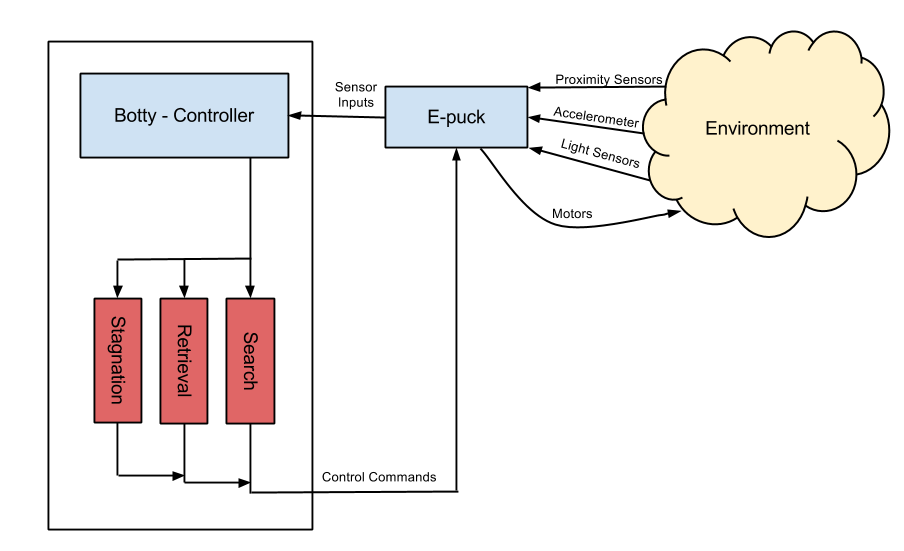
\includegraphics[width=0.8\textwidth]{%
    models/SubSym Proj 4 architecture.png}
  \caption{Controller architecture for the box pushing task.}
  \label{fig:architecture}
\end{figure}

We used the three-layer approach which was used for CRABS, and presented in
the assignment text, but we rewrote each layer from scratch. 
We will not present our initial design for each layer.

\subsection{Search}
The search layer is built as a simple state-based random explorer, which also
tries to avoid crashing into walls.  This layer never supresses (as it is the
most primitive). 

The exploration function is functionally similar to the following pseudo-code:

\begin{python}
def find_speed(self, proximities):
    prox_right, prox_left = proximities[:3], proximities[5:]

    # Check for obstacles
    if any(p > DIST_THRESH for p in prox_right+prox_left):
        tot         = sum(prox_right + prox_left)
        left_power  = sum(prox_left)  / tot
        right_power = sum(prox_right) / tot
        return left_power, right_power
    else:
        # No obstacles, continue in set random direction,
        # or, with random probability, choose a new direction
        if random() < PROB_CHANGE_DIR:
            self.rand_move_dir = (
                uniform(.5, 1.0), 
                uniform(.5, 1.0)
            )
        return self.rand_move_dir
\end{python}

The gist of the code is: If there are obstacles nearby, the bot should try
to avoid them. Otherwise, it will just continue in a set random motion, with
some chance of choosing a new direction (with our current parameter choice, a
direction change can be expected after 2-3 seconds). 

\subsection{Retrieval}
The search layer is the most primitive.
TODO TODO

\subsection{Stagnation}
The search layer is the most primitive.
TODO TODO
TODO TODO
TODO TODO
TODO TODO


\subsection{Resulting behavior}

\section{Possible improvements}
\label{sec:b1}

\section{Implementating and evaluating the improvements}

\begin{figure}[!h]
    \centering

    \begin{subfigure}[!h]{0.45\textwidth}
        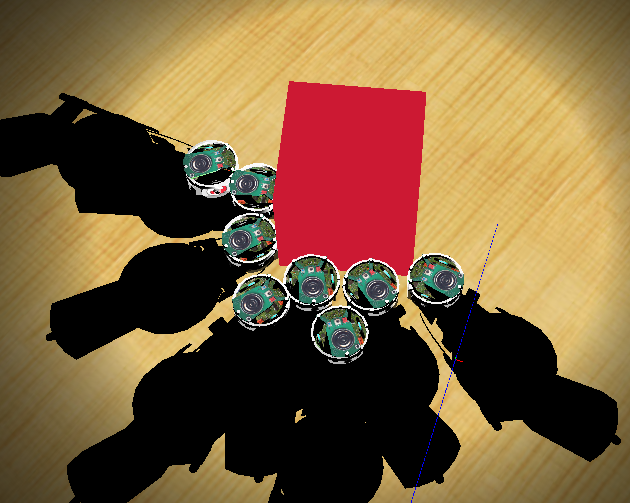
\includegraphics[width=\textwidth]{models/stresstest.PNG}
    \end{subfigure}
    \begin{subfigure}[!h]{0.45\textwidth}
        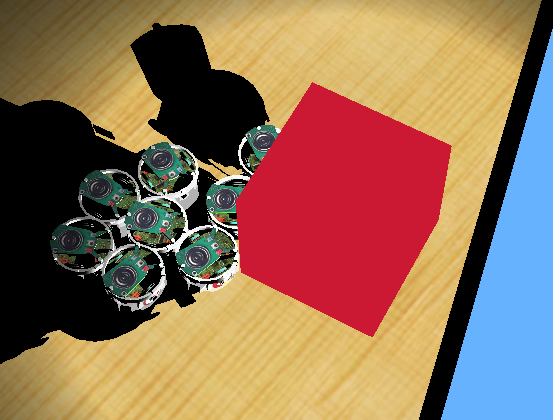
\includegraphics[width=\textwidth]{models/stresstest2.PNG}
    \end{subfigure}

    \caption{A group of eight e-pucks solving a $0.7$-mass box pushing task.
    To move a box with this mass, almost all the robots must take part in the
    pushing motion, and no robot can hinder it.}
\end{figure}


\label{sec:b2}


\end{document}
